\section{Background}\label{sec:background}
\subsection{Preprocessing}

\subsubsection{Standard Scaler}

\subsubsection{Max Absolute Scaler}

\subsubsection{MinMax Scaler}

\subsubsection{Robust Scaler}

\subsubsection{Norm 3}
As previously mentioned, the \gls{chemcam} instrument consists of three spectrometers, each producing 2048 channels.
For data normalization, we follow the approach taken by the SuperCam team and normalize across individual spectrometers' wavelength ranges, a process known as \textit{Norm 3}~\cite{andersonPostlandingMajorElement2022}.
This method ensures that the wavelength intensities captured by each spectrometer is normalized independently.

Figure~\ref{fig:spectral_plot} shows a spectral plot of the \gls{ccs} data for the \textit{ultramafic} sample, illustrating the three distinct spectral regions, each captured by one of the three spectrometers. Specifically, one spectrometer captures the \gls{uv} region, another captures the \gls{vio} region, and the third captures the \gls{vnir} region.

\begin{figure}[H]
	\centering
	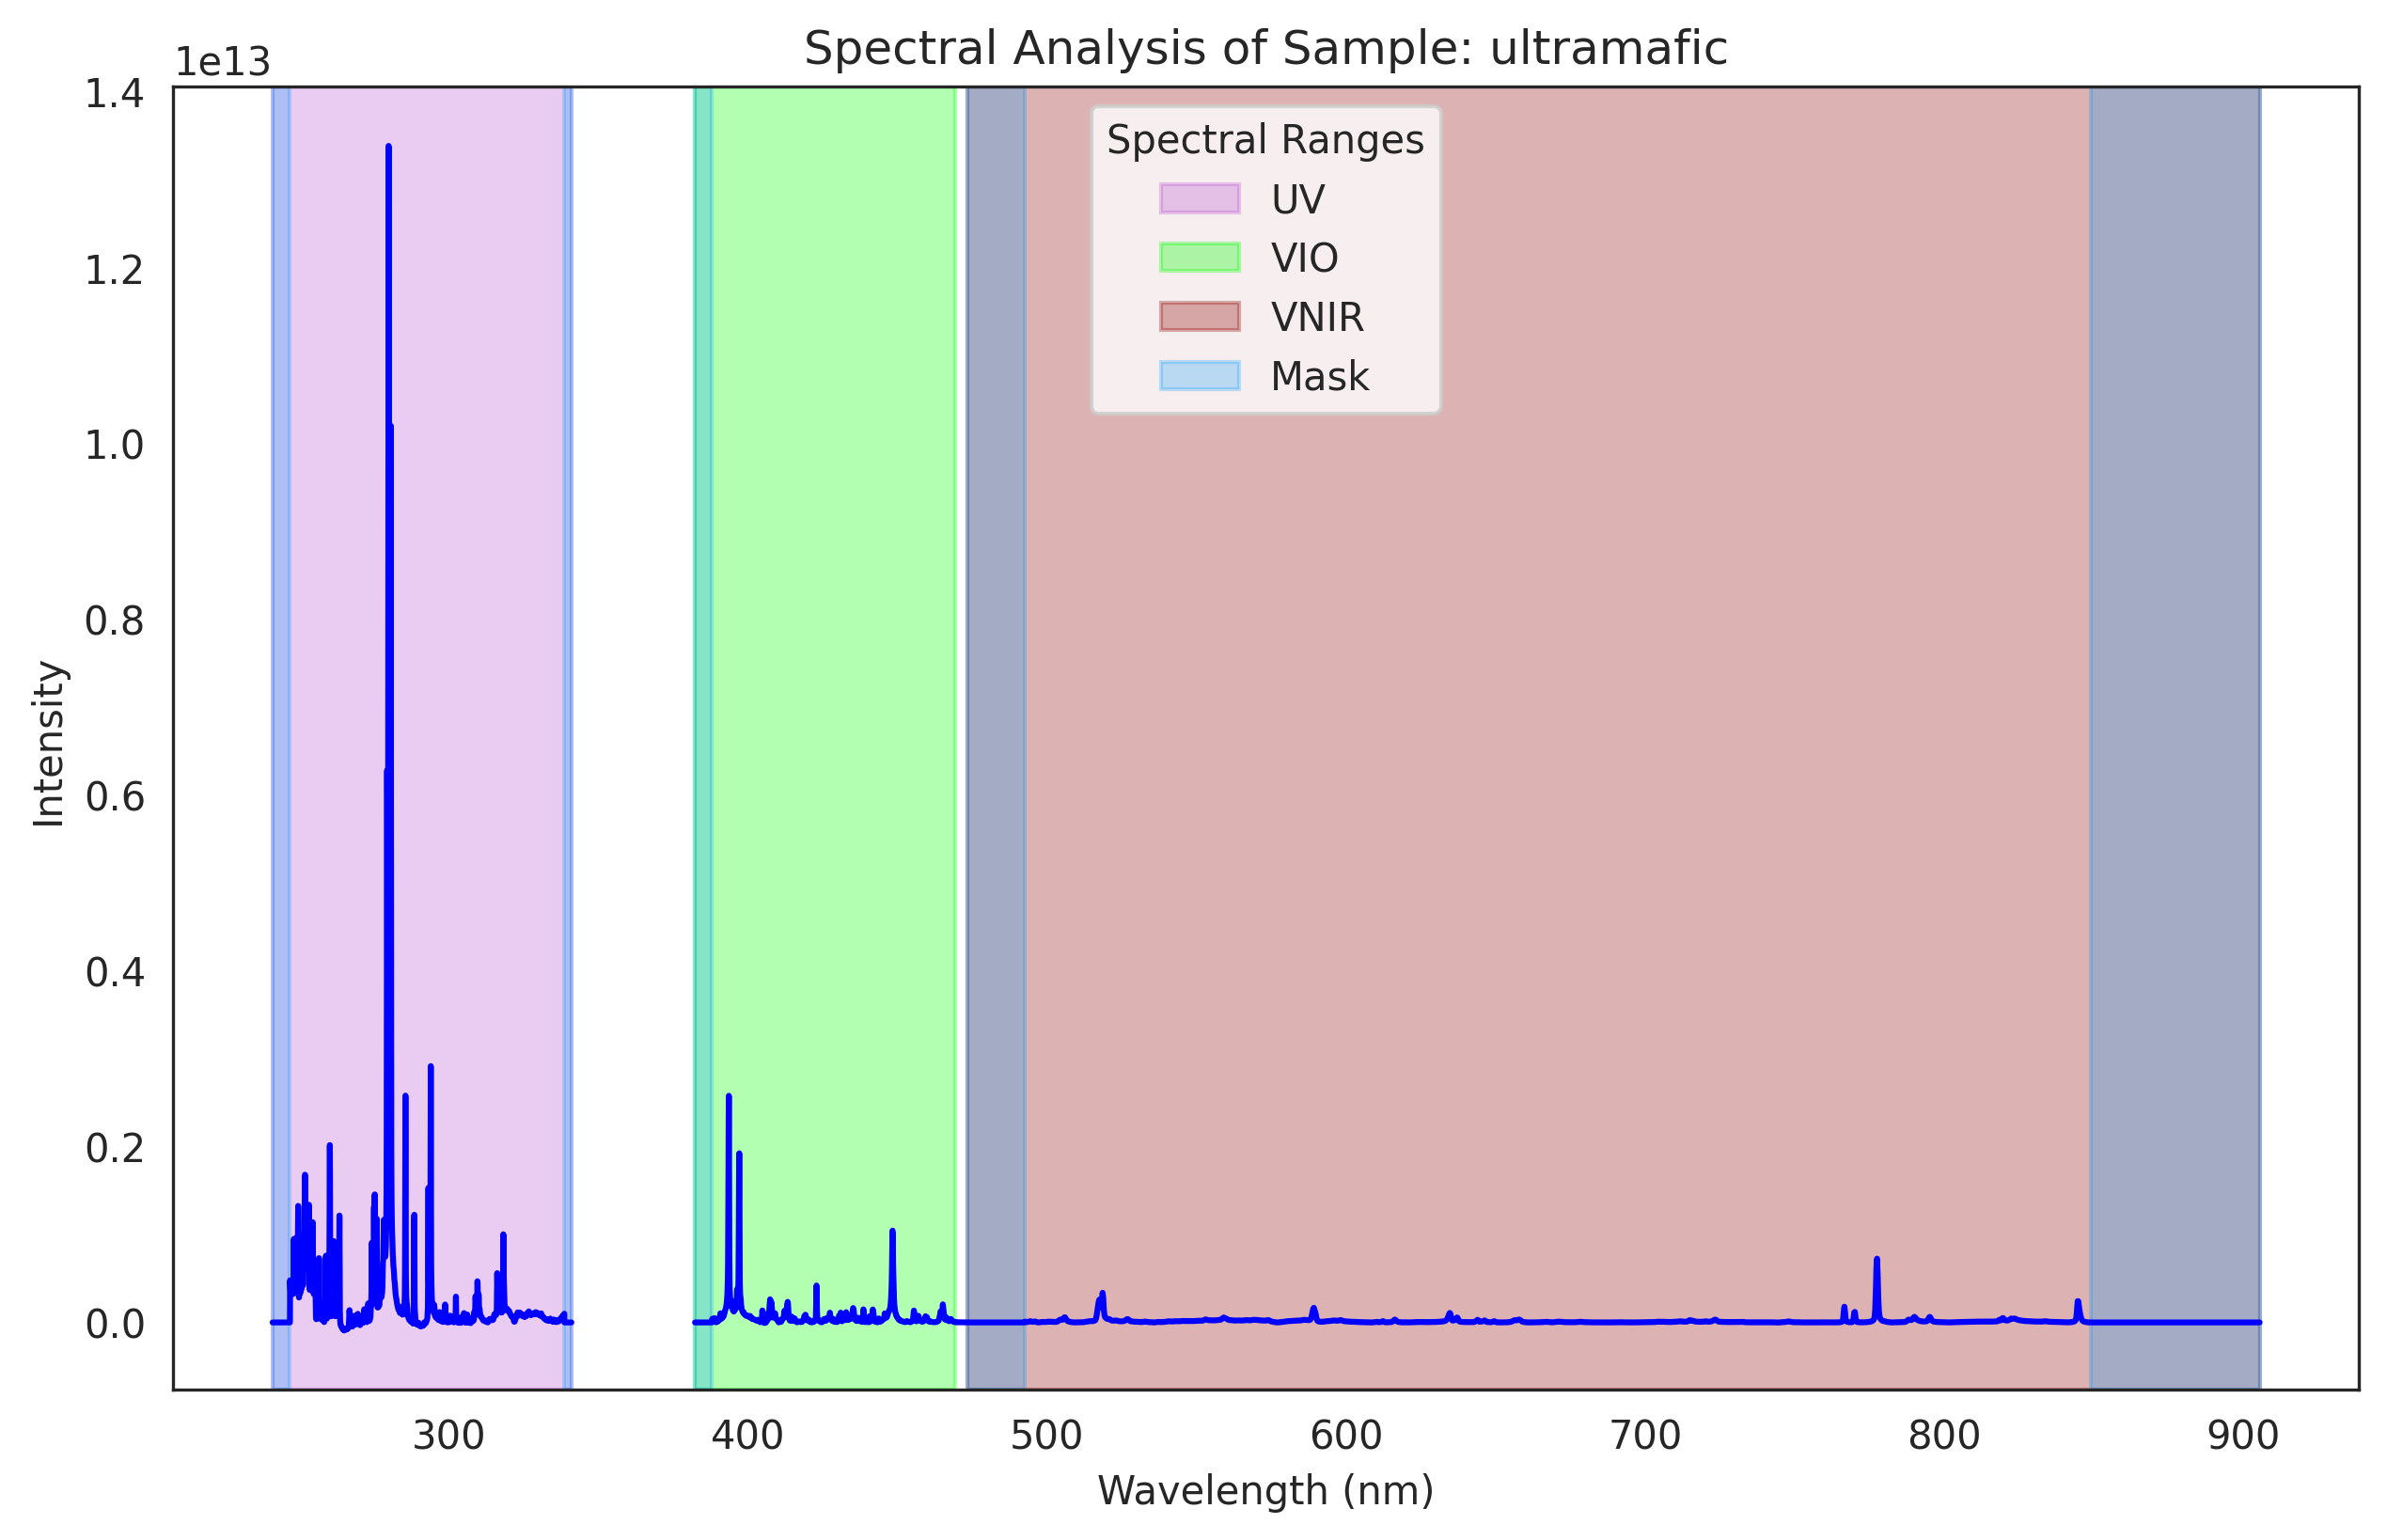
\includegraphics[width=0.5\textwidth]{images/spectral_plot.png}
	\caption{Spectral plot of the \gls{ccs} data for the \textit{ultramafic} sample. The wavelengths represent the spectral channels.}
	\label{fig:spectral_plot}
\end{figure}

Norm 3 can be understood as follows: for each sample, we consider the data from each spectrometer separately. Within each spectrometer, we divide the intensity of each channel by the sum of all channel intensities for that spectrometer. This process is applied for all three spectrometers, resulting in normalized data that preserves the relative intensities within each spectrometer while allowing for comparisons across different samples.

Formally, Norm 3 is defined as

\begin{equation}
	\tilde{X}_{i,j}^{(\gamma)} = \frac{X_{i,j}^{(\gamma)}}{\sum_{j=1}^{N} X_{i,j}^{(\gamma)}},
\end{equation}

where

\begin{itemize}
	\item $\tilde{X}_{i,j}^{(\gamma)}$ is the normalized wavelength intensity for the $i$-th sample in the $j$-th channel on the $\gamma$-th spectrometer with $\gamma \in \{1, 2, 3\}$,
	\item $X_{i,j}^{(\gamma)}$ is the original wavelength intensity for the $i$-th sample in the $j$-th channel on the $\gamma$-th spectrometer,
	\item $N = 2048$ is the number of channels in each spectrometer, and
\end{itemize}

This normalization method results in a total of $3N = 6144$ normalized features for each sample, as each of the three spectrometers contributes 2048 channels.

\subsubsection{Power Transformation}

\subsubsection{Quantile Transformer}

\subsubsection{Principal Component Analysis (PCA)}\label{subsec:pca}
\gls{pca} is a dimensionality reduction technique that transforms a set of possibly correlated variables into a smaller set of uncorrelated variables called \textit{principal components}.
We give an overview of the \gls{pca} algorithm based on \citet{James2023AnIS}.

First, the data matrix $\mathbf{X}$ is centered by subtracting the mean of each variable to ensure that the data is centered at the origin:

$$
\mathbf{\bar{X}} = \mathbf{X} - \mathbf{\mu},
$$

where $\mathbf{\bar{X}}$ is the centered data matrix and $\mathbf{\mu}$ is the mean of each variable.

The covariance matrix of the centered data is then computed:

$$
\mathbf{C} = \frac{1}{n-1} \mathbf{\bar{X}}^T \mathbf{\bar{X}},
$$

where $n$ is the number of samples.

Then, the covariance matrix $C$ is decomposed into its eigenvectors $\mathbf{V}$ and eigenvalues $\mathbf{D}$:

$$
\mathbf{C} = \mathbf{V} \mathbf{D} \mathbf{V}^T,
$$

where matrix $\mathbf{V}$ contains the eigenvectors of $\mathbf{C}$ and represents the principal component loadings.
These loadings indicate the directions of maximum variance in $\mathbf{X}$.
The matrix $\mathbf{D}$ is diagonal and holds the eigenvalues, each of which quantifies the variance captured by its corresponding loading.

These components are the scores $\mathbf{T}$, calculated as follows:

$$
\mathbf{T} = \mathbf{\bar{X}} \mathbf{V}_n,
$$

where $\mathbf{V}_n$ includes only the top $n$ eigenvectors.
The scores $\mathbf{T}$ are the new, uncorrelated features that reduce the dimensionality of the original data, capturing the most significant patterns and trends.

Finally, the original data points are projected onto the space defined by the top $n$ principal components, which transforms $X$ into a lower-dimensional representation:

$$
\mathbf{X}_{\text{reduced}} = \mathbf{\bar{X}} \mathbf{V}_n,
$$

where $\mathbf{V}_n$ is the matrix that only contains the top $n$ eigenvectors.

\subsubsection{Kernel PCA}
We provide a brief overview of the \gls{kernel-pca} algorithm based on \citet{learningwithkernels}.
\gls{kernel-pca} is an extension of traditional \gls{pca} designed to handle nonlinear relationships among data points.
The core idea behind \gls{kernel-pca} is to map data into a higher-dimensional space using a kernel function, a technique known as the kernel trick.
This mapping enables linear separation of data points in the higher-dimensional space, even if they are not linearly separable in the original space.

Similar to \gls{pca}, as described in Section~\ref{subsec:pca}, the goal of \gls{kernel-pca} is to extract the principal components of the data.
However, unlike \gls{pca}, \gls{kernel-pca} does not compute the covariance matrix of the data directly, as it often is infeasible to compute for high-dimensional datasets.
\gls{kernel-pca} instead leverages the kernel trick to computate the similarities between data points directly in the original space using a kernel function $k(\mathbf{x}_i, \mathbf{x}_j)$. 
This kernel function implicitly computes the dot product $\Phi(\mathbf{x}_i)^\top \Phi(\mathbf{x}_j)$ in the higher-dimensional feature space without explicitly performing the mapping. 
By constructing a kernel matrix $\mathbf{K}$ using these pairwise similarities, \gls{kernel-pca} can perform eigenvalue decomposition to obtain the principal components in the feature space, similar to regular \gls{pca} as described in Section~\ref{subsec:pca}.
However, in \gls{kernel-pca}, the eigenvalue decomposition is performed on the kernel matrix $\mathbf{K}$ rather than the covariance matrix $\mathbf{C}$.

\subsection{Overview of Core Models}
In this section, we provide an overview and definitions of \gls{pls}, \gls{svr}, \gls{etr}, \gls{gbr}, and \gls{xgboost}.
These models form the basis of the final architecture of our proposed pipeline, detailed further in Section~\ref{sec:methodology}.

\subsubsection{Partial Least Squares (PLS)}
Having previously introduced \gls{pca}, we now describe \gls{pls} based on \citet{James2023AnIS}.
In order to understand \gls{pls}, it is helpful to first consider \gls{pcr}, as \gls{pls} is an extension of \gls{pcr} that aims to address some of its limitations.

\gls{pcr} extends \gls{pca} in the context of regression analysis.
First, \gls{pca} is applied to the dataset $\mathbf{X}$, transforming it into a set of uncorrelated variables, the principal components.
These components, represented by scores $\mathbf{T}$, are derived from the eigenvectors $\mathbf{V}_n$ with the highest variances.

In \gls{pcr}, the dataset $\mathbf{X}$ is decomposed using PCA as:

$$
\mathbf{X} = \mathbf{TV}^T + \mathbf{E},
$$

where $\mathbf{T}$ represents the scores, and $\mathbf{V}$ represents the loadings.
\gls{pcr} utilizes these scores $\mathbf{T}$ in a linear regression model to predict the target variable $\mathbf{y}$:

$$
\mathbf{y} = \mathbf{Tb} + \mathbf{e},
$$

where $\mathbf{b}$ are the regression coefficients correlating $\mathbf{T}$ to $\mathbf{y}$, and $\mathbf{e}$ is the vector of residuals, capturing the prediction errors.

However, one drawback of \gls{pcr} is that it does not consider the target in the decomposition of the features and therefore assumes that smaller components have a weaker correlation with the target than the larger ones.
This assumption does not always hold, which is what \gls{pls} aims to address.

\gls{pls} uses an iterative method to identify components that maximize the covariance between the features and the target.
These components, $Z$, are linear combinations of the original features, $X_j$, weighted by coefficients, $\phi_j$, which are specifically calculated to reflect this covariance.
The formula for each component is expressed as:

$$
    Z = \sum_{j=1}^{p} \phi_j X_j,
$$

where $Z$ represents the component, $X_j$ is the $j$-th feature, and $\phi_j$ is the weight for the $j$-th feature.
The weights, $\phi_j$, are determined by the formula:

$$
    \phi_j = \frac{\text{cov}(X_j, Y)}{\text{var}(X_j)}.
$$

To refine the model iteratively, PLS uses the residuals from the previous components to calculate the next component.
The $m$-th component, for example, is derived from the residuals of the previous $m-1$ components:

$$
    Z_m = \sum_{j=1}^{p} \phi_{jm} \hat{X}_{j, m-1}.
$$

The components are then used to predict the target variable by fitting a linear model via least squares regression.

\subsubsection{Support Vector Regression (SVR)}
\gls{svr} is a regression technique that extends the principles of \gls{svm} to regression problems.
We therefore provide an overview of \gls{svm}s based on \citet{James2023AnIS} before discussing \gls{svr}s.

\gls{svm} is a supervised learning algorithm used primarily for classification tasks.
A core concept in \gls{svm} is the \textit{hyperplane}.
Generally, a hyperplane is a subspace of one dimension less than its ambient space.
This means that in a two-dimensional space, a hyperplane is a line, while in a three-dimensional space, it is a plane, and so on.

\gls{svm} is built on the idea of finding the hyperplane that best separates the data points into different classes.
This hyperplane is chosen to maximize the margin, which is the distance between the hyperplane and the nearest data point from either class.
The instances right on or inside the margin are called \textit{support vectors}, which are used to 'support' the margin and decision boundary.

\gls{svr} extends the principles of \gls{svm} to regression problems.
We use our previous discussion of \gls{svm} to introduce \gls{svr} based on \citet{druckerSVR}.

\gls{svr} aims to fit a function that predicts continuous values rather than finding the hyperplane that best separates data points.
Instead of using a hyperplane to separate the data, \gls{svr} uses two parallel hyperplanes to define a margin within which the function should lie, often referred to as the $\epsilon$-\textit{tube}, where $\epsilon$ is a hyperparameter that defines the width of the tube.
The goal is to find a function $f(x)$ that lies within this tube and has the maximum number of data points within the tube.
$f(x)$ is typically defined as a linear function of the form:

$$
f(x) = \mathbf{w} \cdot \mathbf{x} + b,
$$

where:

\begin{itemize}
	\item $\mathbf{w}$ is the weight vector,
	\item $\mathbf{x}$ is the input vector, and
	\item $b$ is the bias term.
\end{itemize}

The two parallel hyperplanes at a distance $\epsilon$ from the hyperplane are defined as:

$$
\begin{aligned}
    \mathbf{w} \cdot \mathbf{x} + b &= f(\mathbf{x}) + \epsilon, \\
    \mathbf{w} \cdot \mathbf{x} + b &= f(\mathbf{x}) - \epsilon.
\end{aligned}
$$

Or, more succinctly:

$$
\begin{aligned}
    f^+(\mathbf{x}) &= f(\mathbf{x}) + \epsilon, \\
    f^-(\mathbf{x}) &= f(\mathbf{x}) - \epsilon,
\end{aligned}
$$

where $f^+(\mathbf{x})$ and $f^-(\mathbf{x})$ are the upper and lower bounds of the $\epsilon$-insensitive tube, respectively.

The optimization problem in \gls{svr} is to find the coefficients $\mathbf{w}$ and $b$ that minimize the norm of $\mathbf{w}$ (i.e., keep the regression function as flat as possible) while ensuring that most data points lie within the $\epsilon$ margin.

\subsubsection{Extra Trees Regressor (ETR)}

\subsubsection{Gradient Boosting Regressor (GBR)}

\subsubsection{XGBoost}

\subsection{Stacking Ensemble}
% \citet{pavlyshenko2018stacking}
